\chapter{RESULTADOS}
\label{cap:resultados}

\section{\uppercase{Ambiente e Protocolo Experimental}}

Os métodos foram compilados com g++ 13 (opção \texttt{-O2}) e executados no Ubuntu 24.04 sob o WSL 2, com seis instâncias em paralelo, cada uma em um único núcleo. \textbf{[COMPLETAR: modelo do processador e memória.]} Cada período recebe 3, 4,5 ou 6 segundos de busca, conforme o tamanho da instância, e a fase robusta do período 0 recebe o mesmo limite. Foram usadas as 56 instâncias dos conjuntos A, B, C e X (Tabela~\ref{tab:instancias}).

Todas as soluções foram validadas com o avaliador oficial do desafio (versão 1.2.2), que confere a profundidade máxima, o orçamento de reconfiguração e o atendimento de todas as demandas, e calcula a MLU de cada período. Todas as soluções de AMNS, VND e da solução trivial foram aceitas. Os valores de MLU reportados neste capítulo são os do avaliador oficial e coincidem com os calculados pelos métodos.

Como os métodos param por limite de tempo, execuções diferentes podem produzir resultados ligeiramente diferentes. Os resultados apresentados correspondem a uma única execução de cada método.

\section{\uppercase{Comparação com a Solução Trivial}}

Nos conjuntos A, B e X, a solução trivial, sem \textit{waypoints}, atinge MLU muito próxima de 1: em todas as instâncias exceto setA-02, a MLU do pior período fica entre 0,99997 e 1,00011. Isso indica que as capacidades dessas instâncias foram calibradas para que o roteamento IGP sem otimização sature o enlace mais carregado. Em setA-02, uma intervenção no período 1 leva a carga a 1,098. O conjunto C é diferente: a solução trivial chega a 2,0 em cinco instâncias e a 7,4 em setC-11 e setC-12, ou seja, há enlaces que o roteamento IGP sobrecarrega muito acima da capacidade.

A Tabela~\ref{tab:conjuntos} resume a variação da MLU do pior período em relação à solução trivial, e a Tabela~\ref{tab:resultados} traz os valores por instância. Em média, AMNS e VND reduzem a MLU do pior período em 45,6\% e 45,5\%, respectivamente. As maiores reduções ocorrem nos conjuntos X (65,7\% em média, para ambos) e C (54,0\% e 52,6\%), e as menores no conjunto B (21,3\% e 22,2\%). Nos conjuntos A, B e X, os dois métodos eliminam todas as violações de capacidade. No conjunto C, setC-11 cai de 7,43 para 0,20, mas em cinco instâncias (setC-01, setC-03, setC-04, setC-07 e setC-08) a MLU continua entre 1,15 e 1,25 para os dois métodos, partindo de 2,0 na solução trivial. O avaliador oficial aceita essas soluções, pois a capacidade não é uma restrição rígida; não foi verificado se uma carga abaixo de 1 é possível nessas instâncias. Nesse conjunto o orçamento total é de apenas 46 a 184 segmentos para 24 períodos e milhares de demandas, o que deixa quase todo o trabalho para o período 0.

\begin{table}[H]
\centering
\caption{Variação da MLU do pior período em relação à solução trivial e tempo total, por conjunto.}
\label{tab:conjuntos}
\begin{tabular}{lrrrrrrr}
\toprule
 & & \multicolumn{2}{c}{Média} & \multicolumn{2}{c}{Mediana} & \multicolumn{2}{c}{Tempo total (s)} \\
\cmidrule(lr){3-4} \cmidrule(lr){5-6} \cmidrule(lr){7-8}
Conjunto & Instâncias & AMNS & VND & AMNS & VND & AMNS & VND \\
\midrule
A & 20 & $-$43{,}1\% & $-$43{,}2\% & $-$31{,}6\% & $-$31{,}6\% & 42 & 55 \\
B & 12 & $-$21{,}3\% & $-$22{,}2\% & $-$14{,}1\% & $-$16{,}9\% & 132 & 158 \\
C & 12 & $-$54{,}0\% & $-$52{,}6\% & $-$42{,}7\% & $-$40{,}1\% & 311 & 322 \\
X & 12 & $-$65{,}7\% & $-$65{,}7\% & $-$68{,}7\% & $-$68{,}7\% & 144 & 164 \\
\midrule
Todos & 56 & $-$45{,}6\% & $-$45{,}5\% & $-$42{,}7\% & $-$41{,}1\% & 629 & 699 \\
\bottomrule
\end{tabular}
\end{table}


Em oito instâncias (setA-18, setA-20, setB-02, setB-03, setB-06, setB-08, setB-09 e setB-10) a melhora é menor que 1\%. Nas instâncias que foram analisadas em detalhe, a carga máxima está em enlaces cujo tráfego não pode ser desviado por nenhuma escolha de \textit{waypoints}, como o único enlace de saída da origem de uma demanda. Nesses casos, a MLU de 1 é um limite inferior que nenhum método pode melhorar.

O conjunto C é o mais custoso: 311 segundos para a AMNS e 322 para a VND, cerca de metade do tempo total, contra 72 segundos da solução trivial, cujo tempo é dominado pelo cálculo dos caminhos mínimos nas redes maiores.

A Figura~\ref{fig:resumo} mostra, para cada instância, a MLU do pior período dos três métodos, a variação em relação à solução trivial e o tempo de execução. A Figura~\ref{fig:porconjunto} resume a variação média por conjunto.

\begin{figure}[H]
\centering
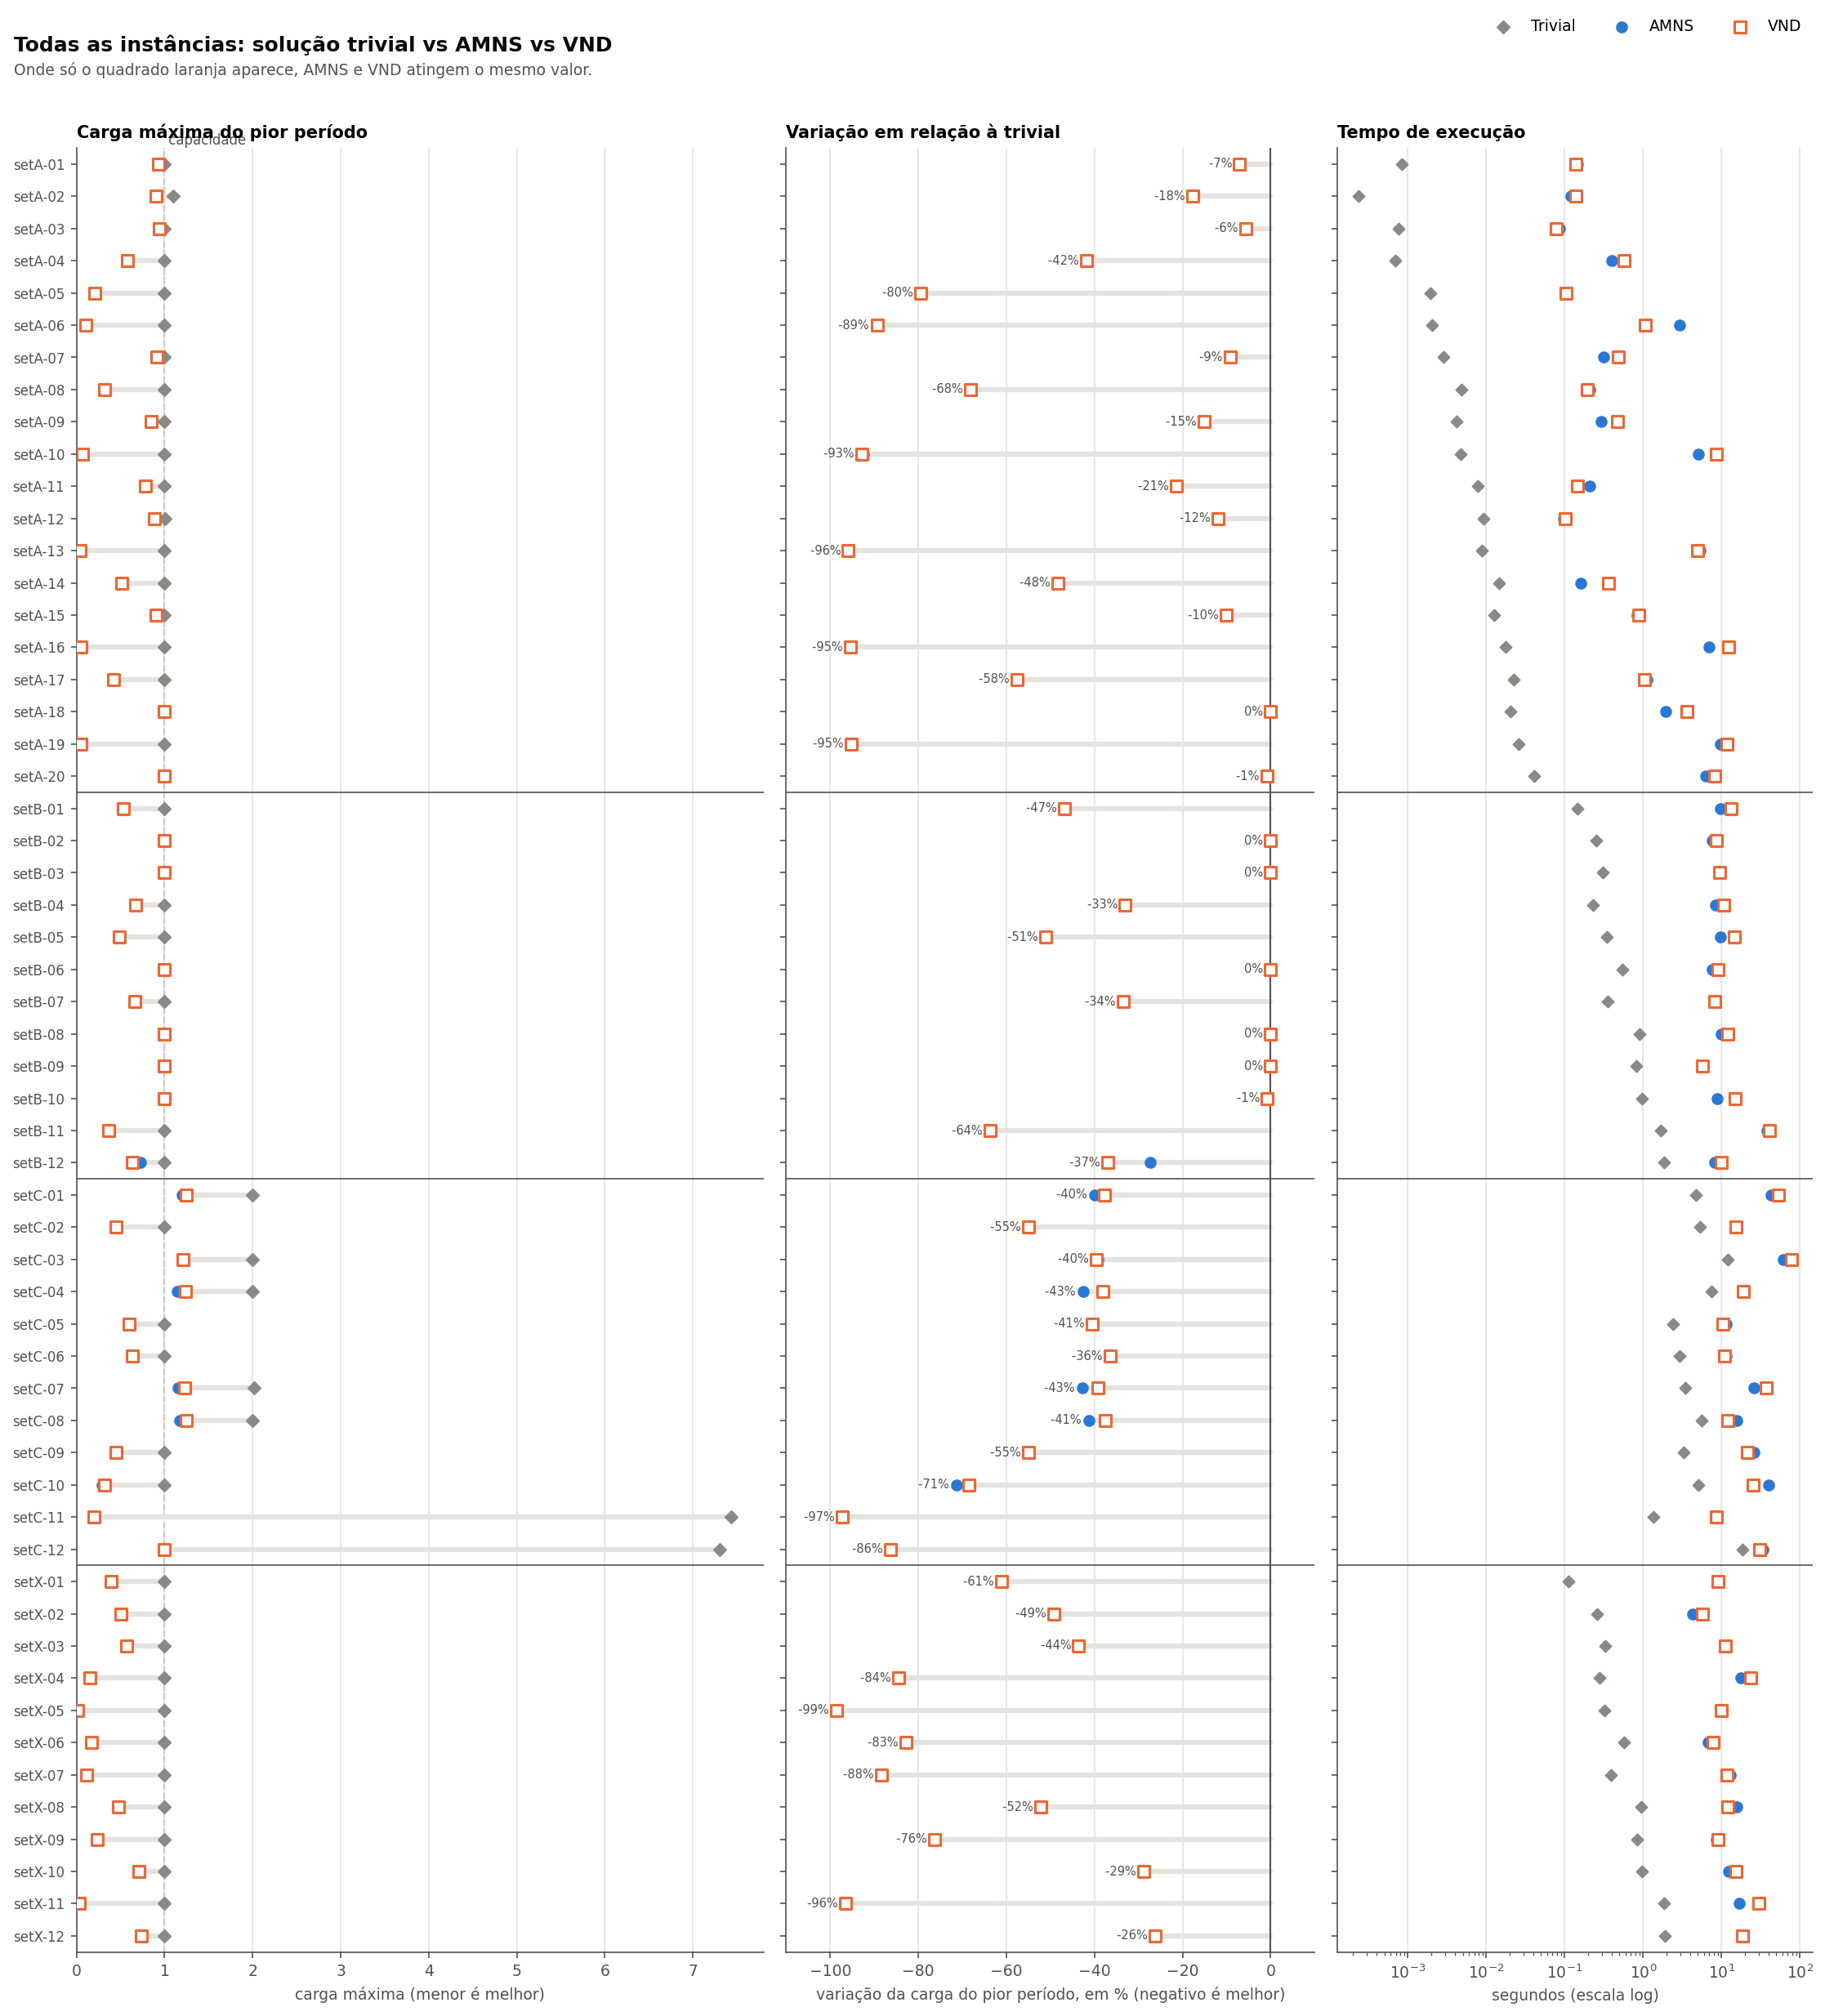
\includegraphics[width=\textwidth]{figuras/resumo_instancias.png}
\caption{MLU do pior período, variação em relação à solução trivial e tempo de execução, por instância. Onde só o quadrado laranja aparece, AMNS e VND atingem o mesmo valor.}
\label{fig:resumo}
\end{figure}

\begin{figure}[H]
\centering
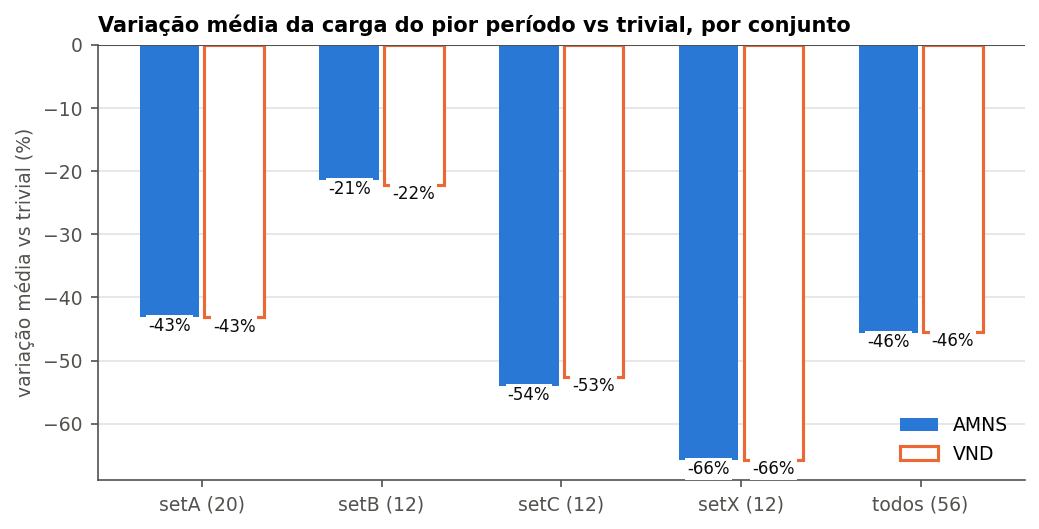
\includegraphics[width=0.75\textwidth]{figuras/resumo_conjuntos.png}
\caption{Variação média da MLU do pior período em relação à solução trivial, por conjunto de instâncias.}
\label{fig:porconjunto}
\end{figure}

\begin{table}[H]
\centering
\caption{MLU do pior período (avaliador oficial) e tempo de execução por instância.}
\label{tab:resultados}
\footnotesize
\begin{tabular}{lrrrrrrr}
\toprule
 & \multicolumn{3}{c}{MLU do pior período} & \multicolumn{2}{c}{Variação vs. trivial} & \multicolumn{2}{c}{Tempo (s)} \\
\cmidrule(lr){2-4} \cmidrule(lr){5-6} \cmidrule(lr){7-8}
Instância & Trivial & AMNS & VND & AMNS & VND & AMNS & VND \\
\midrule
setA-01 & 1{,}000 & 0{,}929 & 0{,}929 & $-$7{,}1\% & $-$7{,}1\% & 0{,}1 & 0{,}1 \\
setA-02 & 1{,}098 & 0{,}903 & 0{,}903 & $-$17{,}8\% & $-$17{,}8\% & 0{,}1 & 0{,}1 \\
setA-03 & 1{,}000 & 0{,}944 & 0{,}944 & $-$5{,}7\% & $-$5{,}7\% & 0{,}1 & 0{,}1 \\
setA-04 & 1{,}000 & 0{,}582 & 0{,}582 & $-$41{,}8\% & $-$41{,}8\% & 0{,}4 & 0{,}6 \\
setA-05 & 1{,}000 & 0{,}205 & 0{,}205 & $-$79{,}5\% & $-$79{,}5\% & 0{,}1 & 0{,}1 \\
setA-06 & 1{,}000 & 0{,}106 & 0{,}107 & $-$89{,}4\% & $-$89{,}3\% & 2{,}9 & 1{,}1 \\
setA-07 & 1{,}000 & 0{,}908 & 0{,}908 & $-$9{,}2\% & $-$9{,}2\% & 0{,}3 & 0{,}5 \\
setA-08 & 1{,}000 & 0{,}319 & 0{,}319 & $-$68{,}1\% & $-$68{,}1\% & 0{,}2 & 0{,}2 \\
setA-09 & 1{,}000 & 0{,}850 & 0{,}850 & $-$15{,}0\% & $-$15{,}0\% & 0{,}3 & 0{,}5 \\
setA-10 & 1{,}000 & 0{,}076 & 0{,}072 & $-$92{,}4\% & $-$92{,}8\% & 5{,}0 & 8{,}6 \\
setA-11 & 1{,}000 & 0{,}786 & 0{,}786 & $-$21{,}4\% & $-$21{,}4\% & 0{,}2 & 0{,}1 \\
setA-12 & 1{,}000 & 0{,}880 & 0{,}880 & $-$12{,}0\% & $-$12{,}0\% & 0{,}1 & 0{,}1 \\
setA-13 & 1{,}000 & 0{,}041 & 0{,}041 & $-$95{,}9\% & $-$95{,}9\% & 5{,}4 & 5{,}0 \\
setA-14 & 1{,}000 & 0{,}518 & 0{,}518 & $-$48{,}2\% & $-$48{,}2\% & 0{,}2 & 0{,}4 \\
setA-15 & 1{,}000 & 0{,}899 & 0{,}899 & $-$10{,}1\% & $-$10{,}1\% & 0{,}8 & 0{,}9 \\
setA-16 & 1{,}000 & 0{,}047 & 0{,}045 & $-$95{,}3\% & $-$95{,}5\% & 7{,}0 & 12{,}4 \\
setA-17 & 1{,}000 & 0{,}424 & 0{,}424 & $-$57{,}6\% & $-$57{,}6\% & 1{,}1 & 1{,}1 \\
setA-18 & 1{,}000 & 1{,}000 & 1{,}000 & 0{,}0\% & 0{,}0\% & 2{,}0 & 3{,}6 \\
setA-19 & 1{,}000 & 0{,}047 & 0{,}047 & $-$95{,}3\% & $-$95{,}3\% & 9{,}7 & 11{,}9 \\
setA-20 & 1{,}000 & 0{,}991 & 0{,}991 & $-$0{,}9\% & $-$0{,}9\% & 6{,}4 & 8{,}2 \\
\midrule
setB-01 & 1{,}000 & 0{,}533 & 0{,}532 & $-$46{,}7\% & $-$46{,}8\% & 9{,}7 & 13{,}2 \\
setB-02 & 1{,}000 & 1{,}000 & 1{,}000 & 0{,}0\% & 0{,}0\% & 7{,}6 & 8{,}7 \\
setB-03 & 1{,}000 & 1{,}000 & 1{,}000 & 0{,}0\% & 0{,}0\% & 9{,}7 & 9{,}6 \\
setB-04 & 1{,}000 & 0{,}670 & 0{,}670 & $-$33{,}0\% & $-$33{,}0\% & 8{,}3 & 10{,}7 \\
setB-05 & 1{,}000 & 0{,}489 & 0{,}489 & $-$51{,}1\% & $-$51{,}1\% & 9{,}6 & 14{,}8 \\
setB-06 & 1{,}000 & 1{,}000 & 1{,}000 & 0{,}0\% & 0{,}0\% & 7{,}6 & 9{,}0 \\
setB-07 & 1{,}000 & 0{,}665 & 0{,}665 & $-$33{,}5\% & $-$33{,}5\% & 8{,}2 & 8{,}2 \\
setB-08 & 1{,}000 & 1{,}000 & 1{,}000 & 0{,}0\% & 0{,}0\% & 9{,}9 & 12{,}0 \\
setB-09 & 1{,}000 & 1{,}000 & 1{,}000 & 0{,}0\% & 0{,}0\% & 5{,}9 & 5{,}7 \\
setB-10 & 1{,}000 & 0{,}992 & 0{,}992 & $-$0{,}8\% & $-$0{,}8\% & 8{,}8 & 15{,}1 \\
setB-11 & 1{,}000 & 0{,}364 & 0{,}364 & $-$63{,}6\% & $-$63{,}6\% & 38{,}4 & 40{,}9 \\
setB-12 & 1{,}000 & 0{,}726 & 0{,}630 & $-$27{,}4\% & $-$37{,}0\% & 8{,}2 & 9{,}8 \\
\midrule
setC-01 & 2{,}000 & 1{,}200 & 1{,}244 & $-$40{,}0\% & $-$37{,}8\% & 42{,}5 & 53{,}5 \\
setC-02 & 1{,}000 & 0{,}450 & 0{,}450 & $-$55{,}0\% & $-$55{,}0\% & 14{,}9 & 15{,}3 \\
setC-03 & 2{,}000 & 1{,}215 & 1{,}207 & $-$39{,}2\% & $-$39{,}6\% & 61{,}5 & 77{,}7 \\
setC-04 & 2{,}000 & 1{,}149 & 1{,}237 & $-$42{,}6\% & $-$38{,}1\% & 18{,}8 & 18{,}9 \\
setC-05 & 1{,}000 & 0{,}594 & 0{,}594 & $-$40{,}5\% & $-$40{,}5\% & 11{,}4 & 10{,}4 \\
setC-06 & 1{,}000 & 0{,}635 & 0{,}635 & $-$36{,}5\% & $-$36{,}5\% & 11{,}6 & 11{,}0 \\
setC-07 & 2{,}015 & 1{,}153 & 1{,}225 & $-$42{,}8\% & $-$39{,}2\% & 26{,}1 & 36{,}9 \\
setC-08 & 2{,}000 & 1{,}174 & 1{,}248 & $-$41{,}3\% & $-$37{,}6\% & 15{,}8 & 12{,}2 \\
setC-09 & 1{,}000 & 0{,}450 & 0{,}450 & $-$55{,}0\% & $-$55{,}0\% & 26{,}2 & 21{,}2 \\
setC-10 & 1{,}000 & 0{,}286 & 0{,}315 & $-$71{,}4\% & $-$68{,}5\% & 40{,}3 & 25{,}4 \\
setC-11 & 7{,}433 & 0{,}200 & 0{,}200 & $-$97{,}3\% & $-$97{,}3\% & 8{,}5 & 8{,}6 \\
setC-12 & 7{,}307 & 1{,}000 & 1{,}000 & $-$86{,}3\% & $-$86{,}3\% & 33{,}7 & 30{,}8 \\
\midrule
setX-01 & 1{,}000 & 0{,}388 & 0{,}388 & $-$61{,}2\% & $-$61{,}2\% & 9{,}2 & 9{,}1 \\
setX-02 & 1{,}000 & 0{,}508 & 0{,}508 & $-$49{,}2\% & $-$49{,}2\% & 4{,}3 & 5{,}7 \\
setX-03 & 1{,}000 & 0{,}564 & 0{,}564 & $-$43{,}6\% & $-$43{,}6\% & 11{,}0 & 11{,}2 \\
setX-04 & 1{,}000 & 0{,}155 & 0{,}155 & $-$84{,}5\% & $-$84{,}5\% & 17{,}6 & 23{,}6 \\
setX-05 & 1{,}000 & 0{,}014 & 0{,}014 & $-$98{,}6\% & $-$98{,}6\% & 9{,}8 & 9{,}9 \\
setX-06 & 1{,}000 & 0{,}172 & 0{,}172 & $-$82{,}8\% & $-$82{,}8\% & 6{,}8 & 7{,}7 \\
setX-07 & 1{,}000 & 0{,}117 & 0{,}117 & $-$88{,}3\% & $-$88{,}3\% & 13{,}1 & 11{,}8 \\
setX-08 & 1{,}000 & 0{,}479 & 0{,}479 & $-$52{,}1\% & $-$52{,}1\% & 15{,}8 & 11{,}9 \\
setX-09 & 1{,}000 & 0{,}238 & 0{,}238 & $-$76{,}2\% & $-$76{,}2\% & 8{,}5 & 9{,}1 \\
setX-10 & 1{,}000 & 0{,}711 & 0{,}711 & $-$28{,}9\% & $-$28{,}9\% & 12{,}4 & 15{,}3 \\
setX-11 & 1{,}000 & 0{,}035 & 0{,}035 & $-$96{,}5\% & $-$96{,}5\% & 17{,}0 & 30{,}2 \\
setX-12 & 1{,}000 & 0{,}737 & 0{,}737 & $-$26{,}3\% & $-$26{,}3\% & 18{,}0 & 18{,}7 \\
\bottomrule
\end{tabular}
\end{table}


\section{\uppercase{Comparação entre AMNS e VND}}

AMNS e VND atingem a mesma MLU do pior período em 43 das 56 instâncias; a AMNS é melhor em 7 (cinco delas no conjunto C) e a VND em 6. A semelhança se explica pela fase robusta, compartilhada pelos dois métodos: como os orçamentos impedem mudanças relevantes depois do período 0, o resultado final é determinado em grande parte pelo planejamento do período 0 feito por essa fase.

O tempo total é de 629 segundos para a AMNS e 699 segundos para a VND; nos conjuntos A, B e X, sem o conjunto C, são 318 e 377 segundos. Em uma versão anterior, a AMNS só parava após 400 chamadas de vizinhança sem nova melhor solução, e qualquer melhora nos critérios de desempate reiniciava essa contagem; nos períodos após o primeiro, em que quase nada pode ser melhorado, ela gastava em média 749 chamadas por período contra 89 da VND, e o tempo total nos conjuntos A, B e X era de 557 segundos. Com a parada após 100 chamadas sem progresso na carga máxima, esse tempo caiu para cerca de 210 segundos, com o mesmo resultado em 40 das 44 instâncias.

A Figura~\ref{fig:overview} detalha a instância setA-02. A solução trivial ultrapassa a capacidade no período 1, após uma intervenção, enquanto AMNS e VND mantêm os dois períodos abaixo de 1. O painel dos 30 enlaces mais carregados mostra o efeito da otimização: as cargas dos enlaces mais carregados caem, ao custo de um pequeno aumento da carga média, porque os desvios alongam as rotas.

\begin{figure}[H]
\centering
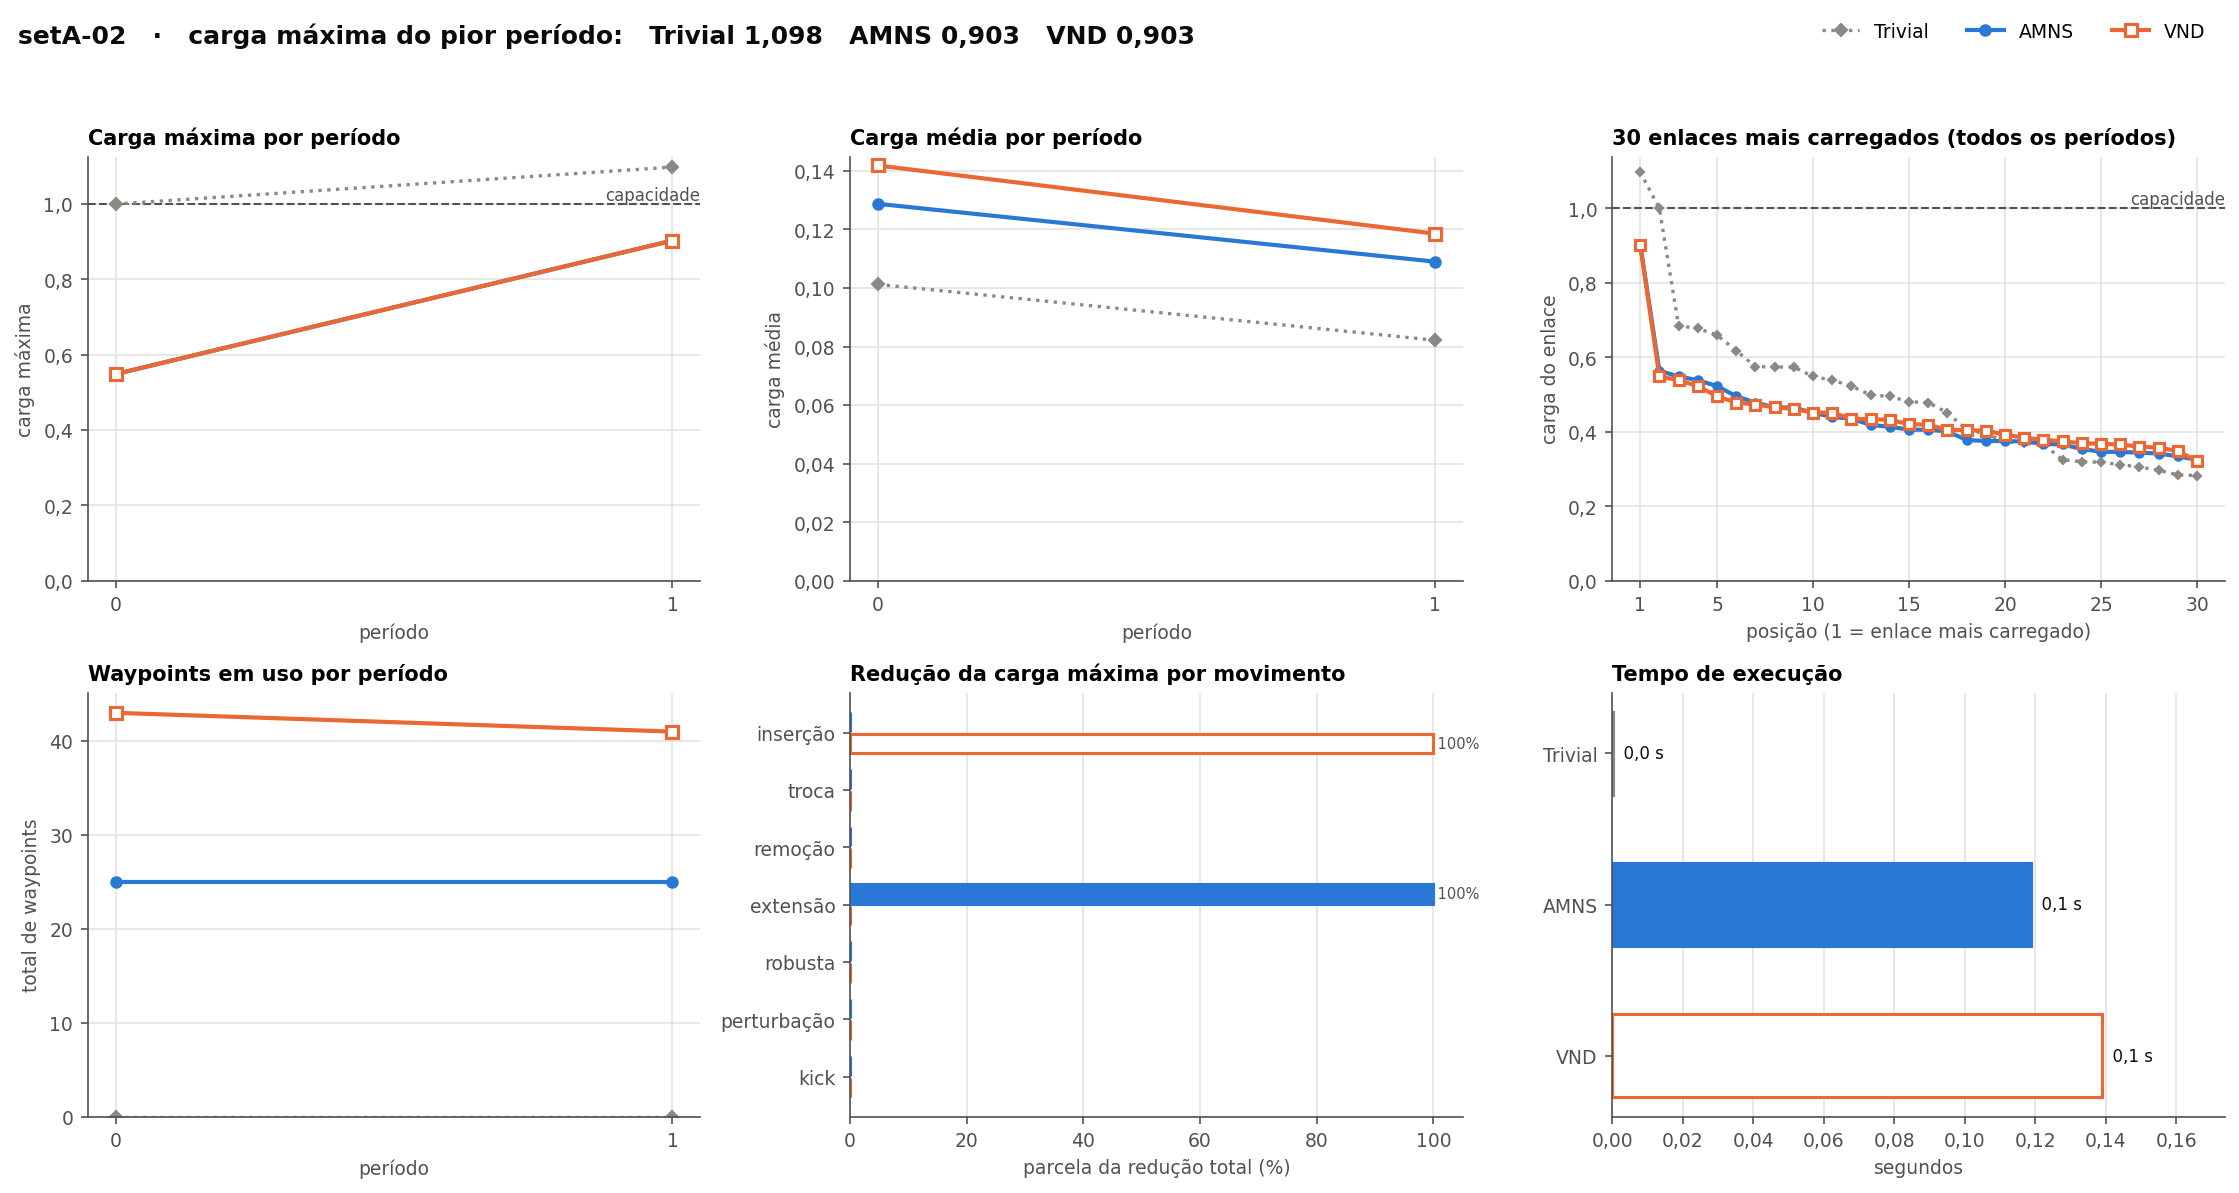
\includegraphics[width=\textwidth]{figuras/setA-02_visao_geral.png}
\caption{Instância setA-02: MLU e carga média por período, 30 enlaces mais carregados, \textit{waypoints} em uso, redução da MLU por movimento e tempo de execução.}
\label{fig:overview}
\end{figure}

A Figura~\ref{fig:historico} mostra a evolução da busca na instância setB-05. A maior parte da redução ocorre no período 0, nas primeiras iterações; nos períodos seguintes, o orçamento permite apenas pequenos ajustes, e só o período 9 apresenta melhora.

\begin{figure}[H]
\centering
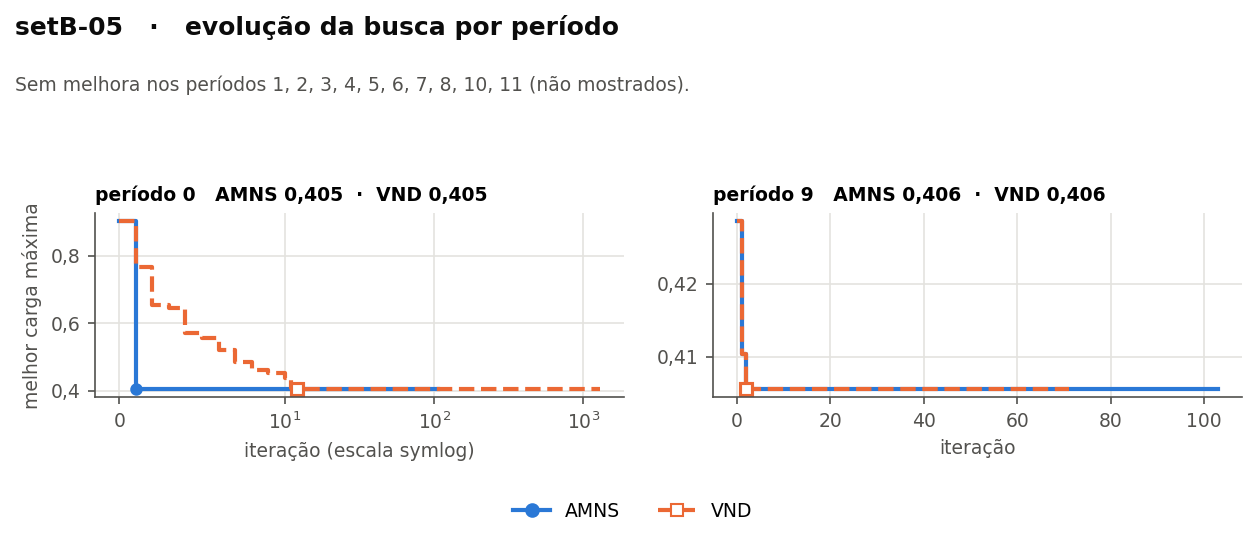
\includegraphics[width=\textwidth]{figuras/setB-05_historico.png}
\caption{Instância setB-05: evolução da melhor MLU ao longo da busca, nos períodos em que houve melhora.}
\label{fig:historico}
\end{figure}

\section{\uppercase{Inserção Dupla de \textit{Waypoints}}}
\label{sec:insercao_dupla}

Foi testado um movimento adicional, a inserção dupla, que insere dois \textit{waypoints} de uma vez em um segmento que atravessa o corte crítico. A motivação é o caso em que um único \textit{waypoint} não resolve: todos os caminhos mínimos até o nó de desvio útil passam pelo próprio enlace congestionado, e só um par $(x, y)$ consegue alcançar $y$ pelo outro lado. Os primeiros \textit{waypoints} $y$ candidatos são os vizinhos dos extremos de cada enlace crítico (outros vizinhos de entrada do nó de chegada e outros vizinhos de saída do nó de partida) e os 6 melhores nós de desvio pela carga residual; para cada $y$, os parceiros $x$ são os 6 melhores nós de desvio antes ou depois de $y$. Na AMNS o movimento recebeu peso inicial 1; na VND foi colocado logo após a inserção simples.

As 56 instâncias foram resolvidas com e sem o movimento, nas mesmas condições. A Tabela~\ref{tab:insercao_dupla} resume o resultado, considerando iguais as diferenças de MLU menores que 0,5\%.

\begin{table}[H]
\centering
\caption{Efeito da inserção dupla: instâncias em que a MLU do pior período melhora ou piora mais de 0,5\%, variação média e tempo total.}
\label{tab:insercao_dupla}
\begin{tabular}{lrrrrr}
\toprule
Método & Melhora & Piora & Variação média & Tempo sem (s) & Tempo com (s) \\
\midrule
AMNS & 4 & 5 & $-$0{,}06\% & 629 & 1987 \\
VND & 0 & 5 & $+$0{,}65\% & 699 & 2343 \\
\bottomrule
\end{tabular}
\end{table}

O movimento não compensa. Na AMNS, os ganhos (setB-12 $-$11,3\%, setC-10 $-$10,7\%, setC-01 $-$5,0\%, setC-03 $-$3,7\%) são anulados pelas perdas (setA-16 $+$13,0\%, setA-06 $+$6,7\%, setC-07 $+$5,2\%), e na VND só há perdas. O tempo total aumenta cerca de 3,2 vezes na AMNS e 3,4 vezes na VND, porque cada chamada avalia dezenas de pares: nos períodos após o primeiro, a inserção dupla consumiu cerca de 1400 segundos na AMNS e 1600 na VND, com menos de 1\% de chamadas bem-sucedidas, enquanto a inserção simples consumiu cerca de 25 segundos. No período 0 ela melhora a solução em 17\% das chamadas na AMNS, mas a inserção simples já faz a maior parte do trabalho, e a fase robusta já usa desvios com dois \textit{waypoints}. As perdas vêm do tempo tirado das outras vizinhanças: com o mesmo limite de tempo por período, sobram menos iterações para a inserção simples e a perturbação. Por isso, a inserção dupla ficou desativada na versão final dos métodos, e todos os demais resultados deste capítulo foram obtidos sem ela.

\section{\uppercase{Tamanho das Listas de Candidatos}}
\label{sec:listas_candidatos}

Os tamanhos das listas de candidatos (16 nós por posição, 32 no período 0, 64 para as demandas no pico da fase robusta e 48 demandas por chamada da extensão e da fase robusta) são fixos, independentemente do tamanho da instância. Foi testada uma regra que os torna proporcionais à instância: cada lista de nós passa a ser uma fração do número de nós $N$ (4\% de $N$ para a lista principal, 8\% no período 0, 16\% para as demandas no pico da fase robusta), e a janela de demandas passa a ser 1\% do número de demandas, com limites inferior e superior. Para $N = 400$, o maior tamanho de rede do conjunto A, a regra reproduz os tamanhos fixos.

Foram avaliadas duas versões nas 56 instâncias. Na primeira, as listas crescem até 3 vezes os tamanhos fixos nas redes grandes. A qualidade praticamente não mudou (variação média da MLU do pior período de $+$0,37\% na AMNS e $-$0,08\% na VND), mas o tempo total aumentou cerca de 47\% (de 629 para 926 segundos na AMNS e de 699 para 942 na VND), quase todo no conjunto C, cujas redes de 800 a 3900 nós atingem os limites superiores. Como o tempo por período é fixo, listas mais longas significam menos iterações, e as duas coisas se compensam. Na segunda versão, os limites superiores são os tamanhos fixos, de modo que as listas só diminuem nas redes pequenas. Nos conjuntos B, C e X, cujas redes são em geral maiores, as listas ficam quase sempre nos tamanhos fixos e o resultado é praticamente o da versão fixa; no conjunto A o efeito é misto: setA-10 e setA-16 melhoram de 4\% a 6\%, mas setA-02, com 30 nós, piora 21,6\% na AMNS, nas duas versões. Como as instâncias pequenas são resolvidas em menos de um segundo, reduzir suas listas não economiza tempo útil.

Esses experimentos também mostram a variabilidade de execuções únicas com limite de tempo: em setC-10, cujos tamanhos de lista são idênticos nas versões fixa e limitada, a MLU variou cerca de 16\% entre as execuções, com os dois métodos. Diferenças desse porte em instâncias isoladas não são, portanto, significativas. Como nenhuma das versões melhorou o resultado médio, os tamanhos fixos foram mantidos.

\section{\uppercase{Discussão}}

Os resultados mostram que o \textit{Segment Routing} reduz substancialmente a carga máxima mesmo com poucos \textit{waypoints} por demanda e com orçamentos de reconfiguração muito restritos. Três observações orientam a continuidade do trabalho:

\begin{itemize}
    \item \textbf{O período 0 decide o resultado.} Com orçamentos pequenos, as rotas do período 0 valem para todo o horizonte. Planejá-las considerando as intervenções futuras foi o fator que mais contribuiu para os resultados.
    \item \textbf{Decisões míopes nos períodos seguintes.} Nos períodos após o primeiro, cada movimento é avaliado apenas pela carga do próprio período, mas suas mudanças permanecem nos períodos seguintes. Na instância setB-12, mudanças feitas nos períodos 2 e 3 elevaram a MLU dos períodos 4 a 7 de 0,630 para 0,726 em uma das execuções da AMNS.
    \item \textbf{AMNS e VND são equivalentes neste contexto.} Como a fase robusta domina o resultado, a escolha entre as duas estratégias de busca afeta mais o tempo de execução do que a qualidade final.
\end{itemize}
